%! TEX root = thesis.tex
\chapter{Problem Formulation, Data and Implementation}%
\label{sec:problemdataimplementation}

Till now, we have got an understanding of the theoretical components that will be used within our research studies and the domains that are of interest to solve this problem. In this chapter, we will formalize the problem statement and understand our evaluation strategy. We will also explore the DALI dataset, with details of how it will be processed to be made use within our Song Lyrics Transcription research. We will briefly touch upon the Software and Hardware ecosystem that we will employ for running experiments for this project. This chapter will be a set the foundational requirements for the implementation methodology (software and hardware), dataset downloading and transformation for usage within the Songs Lyrics Transcription project. In the next chapter, we will directly jump into the research study.


\section{Problem Formulation}%
\label{sec:problemformulation}

The goal of the project is to be able to successfully transcribe songs into lyrics. Given a dataset $D$, where $D = (A_n,T_n)$,  we want to maximize the probability of the predicted class within the lyrics transcription space $P_{o,c}$ to be $y_{o,c}$, given the context of audio signal $A_n$. 

In this scenario, we will aim to create a model that can approximate the function $T_{hat} = F_t(A_n)$ such that the loss  $\sum_{o=1}^N \sum_{c=1}^C loss(y, T_{hat})$ is minimum. In practical terms, since this is a multi-class classification problem at every step, this can be represented as the Cross Entropy Loss provided by the given formula:

\begin{equation}
 {C{e}} = -\sum_{o=1}^N \sum_{c=1}^My_{o,c}\log(p_{o,c}) 
\end{equation}

$where : $

\begin{itemize}
    \item $A_N$ = $A_{1},A_2,A_3,A_4,...., A_n$ represents the audio signals of the format $A = (C,S)$, 
    \item $T_N$ = $T_1,T_2,T_3,T_4,....,T_n$ represents the transcriptions for the corresponding audio signal
    \item $C$ is the number of channels present in the audio
    \item $S$ is the audio signal and of format $S = (X,t)$
    \item $X$ is the array representations of the actual audio track
    \item $t$ is the time component of the audio track
    \item $M$ - number of classes
    \item $log$ - natural log 
    \item $y$ - Actuals (binary flag that indicates if class label $c$ is the correct classification for observation $o$)
    \item $p$ - Predictions (predicted probability for observation $o$ is of class $c$)
    \item $N$ is the number of observations within the dataset.
\end{itemize}


\section{Evaluation Methodology}%
\label{sec:evaluationmetric}

Word Error Rate \cite{zechner2000minimizing} is the edit distance between reference transcription $T$ and its predicted transcription $T_{hat}$. This is a normalized distance as 
it is normalized by the length of the reference transcription. This is a commonly used within Automatic Speech Recognition (ASR) research \cite{zechner2000minimizing} \cite{baevski2020wav2vec} \cite{mccowan2004use}  and is also applied to the Lyrics Transcription domain \cite{ou2022transfer} \cite{gu2022mm}. The metric is calculated as the minimum number of insertions, deletions and substitutions (edit distance) that are required to convert the predicted transcription to the reference transcription. Additionally, the metric involves normalization to be applied in order to be able to compare between different systems or tasks. We will be evaluating the Songs to Lyrics Transcription space with the Word Error Rate (WER) metric as it is the standard measure in similar problems \cite{ou2022transfer} \cite{xu2021self}. Word Error Rate ($WER$) can be calculated as below: 

$$
W E R=\frac{I + D + S}{N}=\frac{I+D+S}{C+D+S}
$$
where

\begin{itemize}
    \item $I$ is the number of insertions,
    \item $D$ is the number of deletions,
    \item $S$ is the number of substitutions,
    \item $C$ is the number of correct words (predicted and actual),
    
    \item $N$ is all the words , i.e, $(\mathrm{N}=\mathrm{S}+\mathrm{D}+\mathrm{C})$
\end{itemize}


\section{Data-set}%
\label{sec:dataset}

\subsection{DALI Data-set}
\label{subsec:dalidataset}

In the project, we will be using the DALI dataset \cite{meseguer2020creating}, which has 5358 audio songs across languages and genres. In this particular dataset, the audio songs have time-matched melody notes and lyrics. Singing Voice, the Music Information Retrieval (MIR) domain under which Song Lyrics Transcription is a part of, is a recent space in spite of the importance of the lyrics and vocals to the songs domain. Earliest works that probe this as a separate topic of interest are quite recent \cite{fujihara2012lyrics} \cite{mesaros2013singing}. Hence, the availability of datasets are limited in this domain, with DALI being one of the largest and diverse datasets that capture this information \cite{ou2022transfer}. The lyrics for DALI dataset are sourced from Karaoke video games, internet etc. As part of the post-processing, they are cleaned, transformed and time aligned through convolution neural network based scoring mechanisms. The dataset itself is not manually annotated by experts and hence cannot be established as a source of truth. In-spite of DALI v2.0 usage by \cite{ou2022transfer}, this is not officially released yet by the owners of the dataset \cite{dalireleases}. Hence, in our study, we retained the more noisier version of the dataset (DALI v1.0). 

\begin{figure}
    \centering
    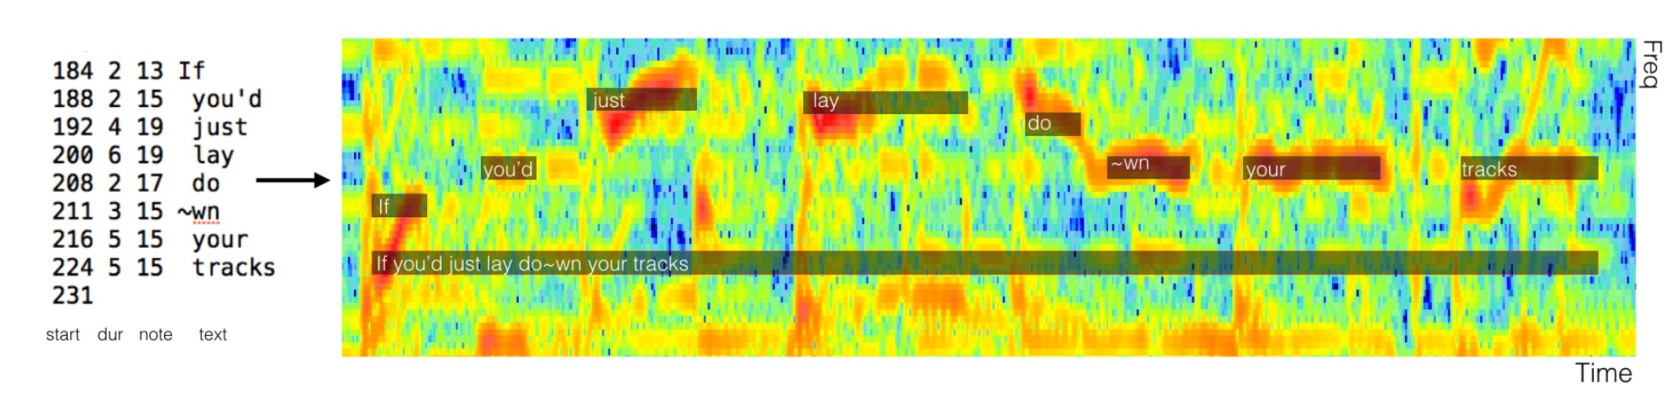
\includegraphics[width=1.0\textwidth]{05-research study/figures/dalidataset.pdf}
    \caption{DALI Data-set}
    \label{fig:dalidataset}
\end{figure}

The dataset doesn't provide access to the audio files directly. The access is provided through a python package developed for DALI. Additionally, the package requires \texttt{youtube-dl}, that downloads the audio files in \texttt{.mp3} files to the hard disk. As part of the project, I have created a python wrapper around the DALI dataset processing to make it easier to use for the project. While the data was downloading, there were several issues that were raised by the downloader, eventually resulting in lesser than advertised audio tracks available for the project. Out of the 5358 audio songs, only 4533 songs were able to be downloaded. The rest of them failed due to the unavailable files, terminated accounts, copyright claims and private files. The 
table \ref{dali-table} provides a breakup of the reported number of audio tracks available in DALI V1.0 and what was eventually available for the project. The entire process to download the data from DALIv1.0 took roughly \textit{10 hours} to fetch the music and store in the local disk.

\renewcommand{\arraystretch}{2}
\setlength{\arrayrulewidth}{0.3mm}
\begin{table}[H]
\small
\begin{center}
\begin{tabular}{ |p{6cm}| p{3cm}| }
\multicolumn{2}{c}{\texttt{DALI Data-set}} \\
\cline{1-2}
 Available vs Reported     & Counts  \\
\hline \hline
 Reported Tracks    & 5358  \\
 File Unavailable   & -315   \\
 Account Terminated & -218   \\
 Copyright Claims   & -148   \\
 Private Files      & -144   \\ 
 \hline \hline
 Total Available    & 4533  \\
 \hline \hline
\end{tabular} 
\caption{\label{dali-table} DALI Data-set - Reported versus Available audio songs}
\end{center}
\end{table}

Within the DALI dataset, audio segments are provided in four granularity levels :

\begin{itemize}
    \item Notes
    \item Words
    \item Lines
    \item Paragraphs
\end{itemize}

The granularity that has been shared above are in increasing level of aggregation. For example, several words together make up a line and several lines make up a paragraph. For each song, additional information such as genre, language, musician, cover and links to video clips are provided through the DALI dataset.For our study, we will ignore the other information and focus only on the audio segments and lyrics themselves.


\subsection{Experiment Setup (Data)}
\label{subsec:datasetup}

The files from YouTube are downloaded in \texttt{.mp3} format. When trying to use it with the \texttt{huggingface} python libraries in the High Performance Computing environment [section \ref{sec:hpc}], there were issues with the \texttt{FFMPEG} plugin not being compatible. To make it work, we used PyDub \cite{robert2018pydub} to convert the files in serial fashion from \texttt{.mp3} to \texttt{.wav} format. This process took roughly \textit{8 hours} to complete. Once the files were converted, they were able to be consumed by \texttt{torchaudio} and \texttt{huggingface} APIs. Within \texttt{huggingface}, we used the \texttt{datasets} and \texttt{transformers} library to process the data. In order to use the audio in a computationally friendly manner, we performed the following additional data setup steps :

\begin{itemize}
    \item Extract the \textbf{lines} granularity from the lyrics and audio segments.
    \item Filter only English songs and discard the rest of the languages
    \item Filter out audio segments that are less than 1 second or greater than 15 seconds
    \item Perform (95\% - 5\%) Train-Test Split. 
    \item Run experiments on Train dataset and evaluate the results on the Test dataset.
\end{itemize}


The reason for limiting the audio to the \textbf{lines} granularity is to ensure that we have more information than a single word as seen in the granularity lower than this one (see section \ref{subsec:dalidataset}). The reason is that this allows for the model to take advantage of the auto-regressive nature of song lyrics, yet not make it computationally expensive by selecting a larger segment of audio and lyrics that can be seen at a \textbf{paragraph} granularity. This is similar to the concept within Whisper model, where the maximum allowed length of an audio segment is 30 seconds. Bigger audio tracks are broken down to smaller chunks and fed to the model. Additionally, the scope of the thesis is only English songs. Hence, songs belonging to other languages have been removed from the dataset. 

When we attempted to use the above audio snippets within our data processing pipelines, our pipelines were constantly stopped because of corrupt audio files. These were removed as part of the data processing step. Similarly, we saw several empty audio segments that were predominantly skewed towards the shorter audio snippets (<1 second). Hence, these were removed. Additionally, we didn't want to have single word occurrence within the lines to ensure our model could learn any auto-regressive property that was needed for it. 

Our final dataset was reduced to 10,045 audio segments that were between 1 to 15 seconds. In order to generate unique identifiers, the audio snippets were named after Universally Unique IDentifier (UUID) hashes by using python's \texttt{uuid} package. The file path of the audio snippets were stored in a \texttt{.csv} file along with the associated lyrics in both uppercase and lowercase form. Since, Wav2vec2 was trained only on uppercase letters, we used the uppercase format for inference for the Wav2Vec2 model. For the Whisper based models, we utilized the lowercase version of the lyrics. The lyrics were cleaned of special characters and made uppercase/lowercase depending on the model. Once the cleaned dataset was present, a train-test split was done. To ensure a high number of audio segments were available while training, a 95\% and 5\% split was done.  The dataset was split into 9538 audio segments being part of the training task and evaluation is done on 507 audio segments. 

In the future, we can increase the scope of the project to cover other languages too and also look to leverage additional information such as singer characteristics and genre to further improve the lyrics transcription. Additionally, we can also incorporate other datasets or manually create datasets to create robust representations.



\section{Hardware Stack}%
\label{sec:hpc}
The experiments for the project were conducted on University of Luxembourg's High Performance Computing (HPC) facility. The experiments were run on the Iris cluster that is based on a Dell/Intel supercomputer consisting of 196 compute nodes (5824 compute cores and 52224 GB RAM) and 24 GPUs ( Nvidia Tesla V100 16GB/32GB) \cite{VBCG_HPCS14}. Our experiments were conducted over 1-4 GPUs (16GB and 32GB versions) and 4-8 CPUs for the data processing parts.

\section{Software Stack}%
\label{sec:softwarestack}

The work leverages PyTorch \cite{paszke2019pytorch} for creating the deep learning architectures. Additionally, we use PyTorch Lightning\cite{Falcon_PyTorch_Lightning_2019} to train models and structuring the experiments in ways that could enable check pointing, logging etc. easily and scale support easily to multiple GPUs. Our work leverages Hugging Face Transformers \cite{wolf-etal-2020-transformers} for accessing pre-trained model and obtaining simpler API that are further abstracted within our code-base. We also used SLURM \cite{yoo2003slurm} for scheduling the work within the Iris super-computing cluster.


\section{Discussion}

In this chapter, we have seen the problem formulation of the research study and the evaluation procedure along with the Word Error Rate (WER) metric. Additionally, we have introduced the DALI dataset and how the DALI dataset is transformed and cleaned from both the audio segments point of view as well as the lyrics before making use of it within the Songs to Lyrics Transcription task. We have also discussed the software and hardware stack that is used for the problem statement and Thesis. In the next chapter, we will follow up with our research study and experiments in view of answering the questions that were outlined in the beginning of the study.